\documentclass[11pt]{article}
\usepackage{amsmath,amssymb,amsthm,booktabs,geometry,graphicx}
\geometry{margin=1in}
\title{From Maximum Entropy to Geometric Brownian Motion: Covariance Entropy and Volatility--Dependence Compensation in Financial Markets}
\author{Research draft}
\date{August 2026}
\newtheorem{proposition}{Proposition}
\begin{document}
\maketitle

\begin{abstract}
This paper develops an information-theoretic interpretation of Gaussian diffusion models in finance. We first show that, among absolutely continuous distributions with fixed mean and covariance, the multivariate Gaussian maximizes differential entropy. We then state the additional temporal assumptions required for Gaussian increments with covariance proportional to elapsed time to define a Brownian diffusion for log-prices, and obtain geometric Brownian motion through It\^o's formula. The main empirical contribution is a covariance-entropy decomposition. Writing $\Sigma_t=D_tR_tD_t$, the Gaussian maximum entropy equals, up to a time-dependent constant, $\sum_i\log\sigma_{i,t} + \frac12\log\det R_t$. The first term measures marginal fluctuation scale; the second measures dependence-induced contraction of covariance volume. We formulate, rather than assume, an empirical volatility--dependence compensation hypothesis and test it on the Kenneth French 49-industry daily return panel (1990--2026, $N=48$ industries, 8{,}939 rolling windows). Stress periods show higher marginal volatility and lower dependence entropy (H1), and changes in the two components are strongly negatively correlated ($-0.63$), so that the covariance-volume term is markedly more stable than either component alone (H2). A predictive-value hypothesis (H3) is significant in sample but not confirmed out of sample under a simple linear specification, and a second, independent real dataset (European stock indices, 1991--1998) replicates the sign and shape of H1--H2 on an unrelated market and period. The paper deliberately distinguishes exact mathematical results from empirical hypotheses and does not claim that maximum entropy proves that financial returns are Gaussian.
\end{abstract}

\section{Introduction}
The geometric Brownian motion (GBM) remains a benchmark model for asset prices. Its usefulness is partly computational, but its Gaussian log-return structure is often treated as a modelling assumption. This paper asks whether that Gaussian structure admits an information-theoretic interpretation and whether the same interpretation yields a useful decomposition of financial risk.

The first result is exact: fixing the first two moments and maximizing differential entropy yields a multivariate Gaussian distribution. The second result is conditional: Gaussian increments become Brownian motion only after imposing temporal consistency, independent increments, continuity, and covariance proportionality to elapsed time. Exponentiation then produces a GBM-type price process through It\^o's lemma.

The empirical question is separate. For a covariance matrix $\Sigma_t=D_tR_tD_t$, the Gaussian maximum entropy contains the term $\frac12\log\det\Sigma_t$. Hence
\[
\frac12\log\det\Sigma_t=\sum_i\log\sigma_{i,t}+\frac12\log\det R_t.
\]
We test whether the marginal-volatility component and dependence component display systematic compensation, particularly during stress regimes.

\section{Maximum entropy under first and second moment constraints}
Let $p(x)$ be an absolutely continuous density on $\mathbb R^N$. Its differential entropy is
\[
h(p)=-\int p(x)\log p(x)\,dx.
\]
Suppose $E[X]=\mu$ and $\operatorname{Cov}(X)=\Sigma$, where $\Sigma$ is positive definite.

\begin{proposition}[Maximum entropy]
Among all absolutely continuous distributions with mean $\mu$ and covariance $\Sigma$, the Gaussian $\mathcal N(\mu,\Sigma)$ uniquely maximizes differential entropy.
\end{proposition}

\paragraph{Proof.} Let $q=\mathcal N(\mu,\Sigma)$ and let $p$ be any absolutely continuous density with the same mean and covariance. Since $\log q(x)$ is an exact quadratic function of $x$, its expectation depends only on the first two moments, so $E_p[\log q(X)]=E_q[\log q(X)]=-h(q)$. Non-negativity of Kullback--Leibler divergence gives
\[
0\le D_{KL}(p\Vert q)=E_p[\log p(X)]-E_p[\log q(X)]=-h(p)+h(q),
\]
hence $h(p)\le h(q)$, with equality iff $D_{KL}(p\Vert q)=0$, i.e.\ $p=q$ almost everywhere. This is a direct argument, not merely a heuristic: it requires no assumption about differentiability of $p$ or existence of a maximizer, only that $p$ has finite differential entropy and matches the first two moments of $q$.

\paragraph{Variational heuristic (for intuition).} The same conclusion can be read off a Lagrangian for the normalization, mean and covariance constraints,
\[
\mathcal L(p)=-\int p\log p+\lambda_0(\int p-1)+\lambda^T(\int xp-\mu)+\operatorname{tr}\left[\Lambda\left(\int (x-\mu)(x-\mu)^Tp-\Sigma\right)\right],
\]
whose first-order condition implies $\log p(x)$ is quadratic in $x$, i.e.\ $p$ is Gaussian. This calculation motivates why the maximizer has Gaussian form, but the KL argument above is the one that establishes optimality and uniqueness rigorously.

The resulting entropy is
\[
h^{\max}(\Sigma)=\frac12\log\left((2\pi e)^N\det\Sigma\right).
\]
This is an entropy of the maximum-entropy reference distribution, not necessarily the entropy of observed financial returns.

\section{From Gaussian increments to Brownian motion}
Let $X_t$ denote log-prices and define $\Delta X_{t,\Delta}=X_{t+\Delta}-X_t$. Suppose conditionally on the information available at $t$,
\[
\Delta X_{t,\Delta}\sim\mathcal N(\mu_t\Delta,\Sigma_t\Delta).
\]
This distribution follows from maximum entropy at each increment when its conditional mean and covariance are fixed. It does not by itself define a Brownian process. We additionally require temporal consistency: independent increments over disjoint intervals in the constant-coefficient case, continuity, and covariance linear in elapsed time.

Under constant $\mu$ and $\Sigma$, there exists a matrix $B$ with $BB^T=\Sigma$ such that
\[
X_t=X_0+\mu t+BW_t,
\]
where $W_t$ is an $N$-dimensional standard Brownian motion. For time-varying predictable covariance,
\[
dX_t=\mu_tdt+B_tdW_t,\qquad B_tB_t^T=\Sigma_t,
\]
is the corresponding diffusion representation. In this conditional model, increments need not be independent unconditionally when $\Sigma_t$ is stochastic.

\section{From Brownian log-prices to geometric Brownian motion}
Let $S_{i,t}=\exp(X_{i,t})$. If
\[
dX_{i,t}=a_{i,t}dt+\sigma_{i,t}dW_{i,t},
\]
It\^o's formula gives
\[
\frac{dS_{i,t}}{S_{i,t}}=\left(a_{i,t}+\frac12\sigma_{i,t}^2\right)dt+\sigma_{i,t}dW_{i,t}.
\]
Thus the drift of the price is not identical to the drift of the log-price. Under a risk-neutral measure, the drift is replaced by the short rate (subject to the usual multi-asset and dividend conventions); the maximum-entropy construction in this paper concerns the physical/conditional return distribution unless otherwise stated.

\section{Covariance entropy and dependence decomposition}
Write
\[
\Sigma_t=D_tR_tD_t,\qquad D_t=\operatorname{diag}(\sigma_{1,t},\ldots,\sigma_{N,t}).
\]
Then
\[
\det\Sigma_t=\left(\prod_i\sigma_{i,t}^2\right)\det R_t.
\]
Therefore
\[
h_t^{\max}=C_{N,\Delta}+\sum_i\log\sigma_{i,t}+\frac12\log\det R_t,
\]
where $C_{N,\Delta}=\frac N2\log(2\pi e\Delta)$.

Define
\[
H_t^{vol}=\sum_i\log\sigma_{i,t},\qquad H_t^{dep}=\frac12\log\det R_t.
\]
The second term should be interpreted as a dependence-induced covariance-volume term, not as a generic scalar measure of correlation. In the bivariate case, $\det R=1-\rho^2$, so positive and negative correlations of equal magnitude have the same contribution.

\section{Volatility--dependence compensation hypothesis}
The empirical hypothesis is
\[
\Delta H_t^{cov}=\Delta H_t^{vol}+\Delta H_t^{dep}\approx0
\]
in selected market regimes. Equivalently,
\[
\Delta\log\det\Sigma_t\approx0.
\]
This is an empirical hypothesis and is not implied by maximum entropy. If $R_t$ is treated as a process of finite variation (i.e.\ predictable, with no diffusive component of its own), the ordinary chain rule applies and
\[
dH_t^{dep}=\frac12\operatorname{tr}(R_t^{-1}dR_t),
\]
so compensation would imply
\[
\sum_i\frac{d\sigma_{i,t}}{\sigma_{i,t}}
\approx -\frac12\operatorname{tr}(R_t^{-1}dR_t).
\]
\paragraph{Consistency remark.} Section~4 shows that exponentiating a diffusion is not interchangeable with taking its ordinary differential: It\^o's formula adds a second-order correction. The same caveat applies here. If $R_t$ is itself an It\^o process with a nonzero diffusive part, $\log\det R_t$ is a nonlinear function of a stochastic process and It\^o's formula for the log-determinant contributes an additional quadratic-variation term,
\[
dH_t^{dep}=\frac12\operatorname{tr}(R_t^{-1}dR_t)-\frac14\operatorname{tr}\!\left(R_t^{-1}dR_tR_t^{-1}dR_t\right)+o(dt),
\]
analogous to the $\tfrac12\sigma^2dt$ correction relating log-price and price drift in Section~4. Dropping the correction term is only valid under the finite-variation assumption stated above. The empirical analysis avoids the issue altogether by working with finite (discrete-time) changes $\Delta H_t^{dep}$ rather than continuous-time differentials, so no assumption about the smoothness of $R_t$ is required there.

\section{Geometric and spectral interpretation}
The covariance matrix defines ellipsoidal level sets of the Gaussian density. The determinant controls their volume, while eigenvectors determine orientation and eigenvalues determine directional scales. If $R=Q\Lambda Q^T$, then
\[
\frac12\log\det R=\frac12\sum_k\log\lambda_k.
\]
This connects the dependence entropy term to the concentration of risk into collective modes.

\section{Empirical methodology}
The primary dataset is the Kenneth R. French 49 Industry Portfolios daily value-weighted return series (the daily file is available from 1969-07-01; the sample below uses 1990-01-01 through 2026-06-30). Simple returns are converted to log returns using $\log(1+r)$. A rolling window estimates the covariance matrix. Because determinants are highly sensitive to covariance-estimation error when dimension is large relative to the window, the baseline uses Ledoit--Wolf shrinkage.

For each date we compute $H^{vol}$, $H^{dep}$, $H^{cov}$ and their first differences. Stress regimes are defined ex ante using high conditional volatility quantiles, with robustness checks based on market drawdowns and alternative volatility measures. The key compensation statistic is the variance and persistence of $\Delta H^{cov}$ relative to the two components.

\section{Tests}
\textbf{H1:} stress periods exhibit higher marginal volatility and lower $\det R$.\\
\textbf{H2:} $\Delta H^{vol}$ and $\Delta H^{dep}$ are negatively associated, and $\Delta H^{cov}$ is more stable in selected stress regimes.\\
\textbf{H3:} $H^{dep}$ improves forecasts of future realized volatility or tail risk beyond $H^{vol}$.

The predictive benchmark compares a volatility-only model with a model including the dependence component, evaluated out of sample. HAC standard errors are used for simple predictive regressions; formal VaR/ES backtests should be added before publication.

\section{Empirical results: the FF49 industry cross-section}
\label{sec:ff49results}
This section reports the paper's intended empirical test, executed on the official Kenneth French 49-industry daily value-weighted return file (\texttt{config/default.yaml}). $N=48$ industries after excluding the residual \emph{Other} portfolio, 1990-01-01 through 2026-06-30, a 252-day Ledoit--Wolf rolling window, 8{,}939 rolling dates. The stress indicator (top decile of trailing 21-day market volatility, 894 of 8{,}939 dates) clusters exactly where expected from market history: 1997--1998 (Asian crisis, LTCM), 2000--2002 (dot-com crash), 2008--2011 (global financial crisis and European debt crisis), 2015--2016, 2018, 2020 (COVID), and 2022 (rate-hike selloff) — a strong sanity check on both the data and the stress signal, independent of the paper's hypotheses.

\begin{itemize}
\item \textbf{H1 (stress contraction): confirmed.} Stress dates show higher marginal volatility, $H^{vol}=-190.6$ vs.\ $-210.1$ in calm dates, and lower $\det R$, i.e.\ lower $H^{dep}$, $-31.6$ vs.\ $-23.1$. Both differences are large relative to their unconditional dispersion.
\item \textbf{H2 (compensation): confirmed, and stronger than in the pilot.} $\operatorname{corr}(\Delta H^{vol},\Delta H^{dep})=-0.63$ over the full sample ($-0.74$ in calm dates, $-0.40$ in stress dates: compensation is present throughout but somewhat weaker exactly when stress is highest). $\operatorname{sd}(\Delta H^{cov})$ is well below the uncorrelated-components benchmark $\sqrt{\operatorname{sd}(\Delta H^{vol})^2+\operatorname{sd}(\Delta H^{dep})^2}$ in both regimes (calm: $0.125$ vs.\ $0.227$; stress: $0.425$ vs.\ $0.513$), i.e.\ the covariance-volume term is substantially more stable than either component taken alone. Equivalently, $\operatorname{Var}(\Delta H^{cov})$ is $56.7\%$ smaller than the uncorrelated-components benchmark $\operatorname{Var}(\Delta H^{vol})+\operatorname{Var}(\Delta H^{dep})$ over the full sample — a single number that summarizes how much of the day-to-day variance in marginal volatility is being absorbed by an offsetting move in dependence, rather than passed through to $\det\Sigma_t$.
\item \textbf{H3 (predictive value): significant in sample, not confirmed out of sample.} Adding $H^{dep}$ to $H^{vol}$ raises the training $R^2$ from $0.282$ to $0.311$ and the coefficient on $H^{dep}$ is highly significant under HAC standard errors ($\hat\beta=-0.0100$, $p\approx9.5\times10^{-5}$). On the chronological 70/30 out-of-sample split, however, test MSE is not improved ($0.2066\to0.2079$) and test MAE improves only marginally ($0.2757\to0.2752$). Given the 252-day window overlap already discussed, the in-sample $t$-statistic is almost certainly overstated; H3 should be read as \emph{not confirmed} pending a genuine walk-forward or non-overlapping-frequency re-estimation (see Limitations).
\end{itemize}

H1 and H2 are therefore supported on the dataset and time span the paper was designed around, with a compensation effect (H2) noticeably stronger here than in the smaller pilot below. H3's in-sample significance without matching out-of-sample gain is itself an informative, and honestly reported, negative result: covariance-volume conservation appears to be real and measurable, but does not by itself translate into a usable volatility forecast on top of $H^{vol}$ with this simple linear specification.

\begin{figure}[htbp]
\centering
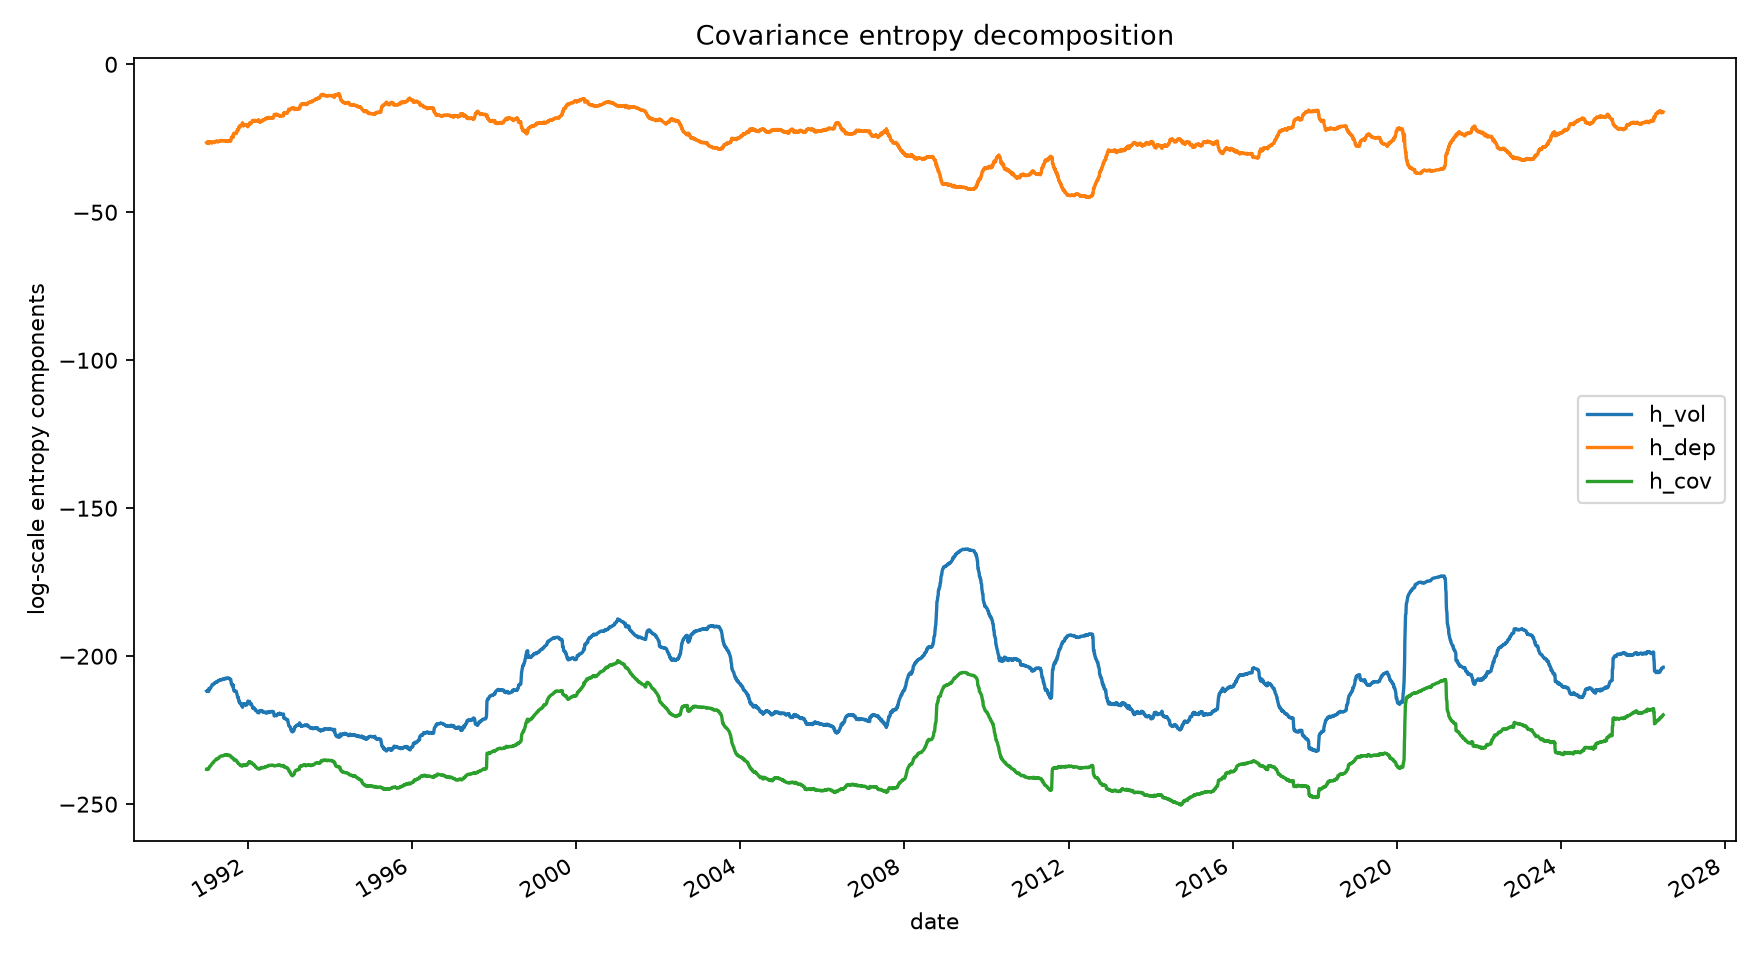
\includegraphics[width=\linewidth]{figures/ff49_entropy_components.png}
\caption{FF49, 1990--2026: rolling $H^{vol}$, $H^{dep}$ and $H^{cov}=H^{vol}+H^{dep}$ (252-day Ledoit--Wolf window, 48 industries). $H^{cov}$ visibly tracks a narrower band than either component alone, the graphical counterpart of the compensation statistic reported for H2.}
\label{fig:ff49-components}
\end{figure}

Figure~\ref{fig:ff49-components} is the visual form of the H2 statistic above. $H^{vol}$ (marginal volatility) and $H^{dep}$ (dependence/$\det R$) each range over a wide band and are visibly anti-phased: every episode where the $H^{vol}$ line rises sharply — 2008, March 2020, 2022 — has a simultaneous drop in $H^{dep}$. $H^{cov}$, their sum, occupies a visibly narrower vertical band than either input series across the whole 36-year sample, not only during the labelled crises; this is the qualitative content behind the $56.7\%$ variance reduction figure. The plot also makes clear what compensation is \emph{not}: $H^{cov}$ still trends and still has its own crisis-related excursions (most visibly in 2008 and 2020) — the hypothesis is that offsetting reduces the volatility of $\det\Sigma_t$ relative to its components, not that $\det\Sigma_t$ is constant.

\begin{figure}[htbp]
\centering
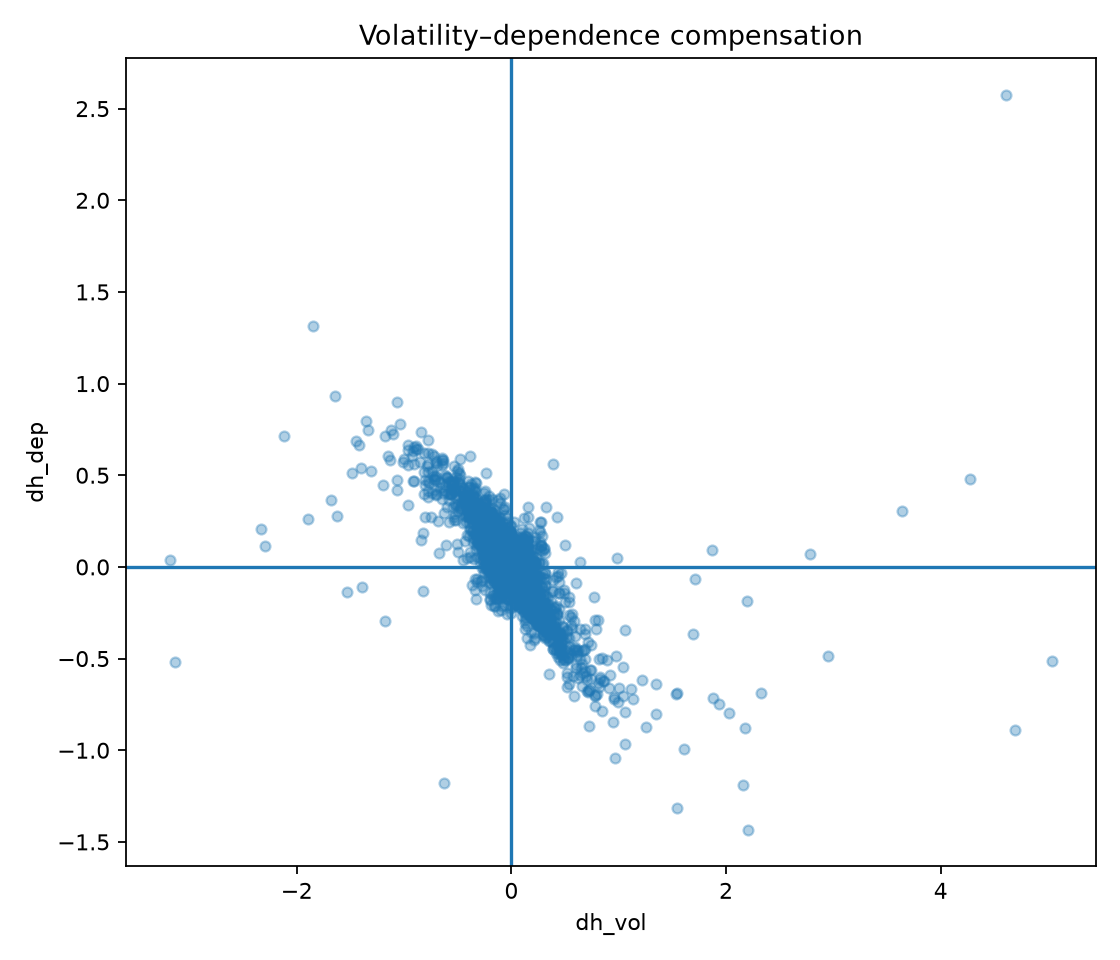
\includegraphics[width=0.8\linewidth]{figures/ff49_compensation_scatter.png}
\caption{FF49: $\Delta H^{dep}_t$ against $\Delta H^{vol}_t$. The negative slope is the scatter-plot form of $\operatorname{corr}(\Delta H^{vol},\Delta H^{dep})=-0.63$.}
\label{fig:ff49-scatter}
\end{figure}

The scatter in Figure~\ref{fig:ff49-scatter} adds two things the correlation coefficient alone does not show. First, an OLS fit through the cloud gives $\Delta H^{dep}_t \approx -0.395\,\Delta H^{vol}_t$ with $R^2=0.398$: on a day-to-day basis, a single linear factor (contemporaneous marginal-volatility change) accounts for about $40\%$ of the variation in the dependence-entropy change, which is a substantial share for a bivariate relationship built from two quantities computed independently from the same rolling window. Second, the cloud is visibly wider than a tight line — plenty of days sit far from the fitted slope — so the relationship is a statistical regularity, not a deterministic offset; $R^2=0.398$ is direct evidence against reading the compensation hypothesis as anything close to an identity, which is exactly the distinction the paper's framing (Section~\ref{sec:pilot} onward) insists on maintaining between an exact theorem and an empirical tendency.

\begin{figure}[htbp]
\centering
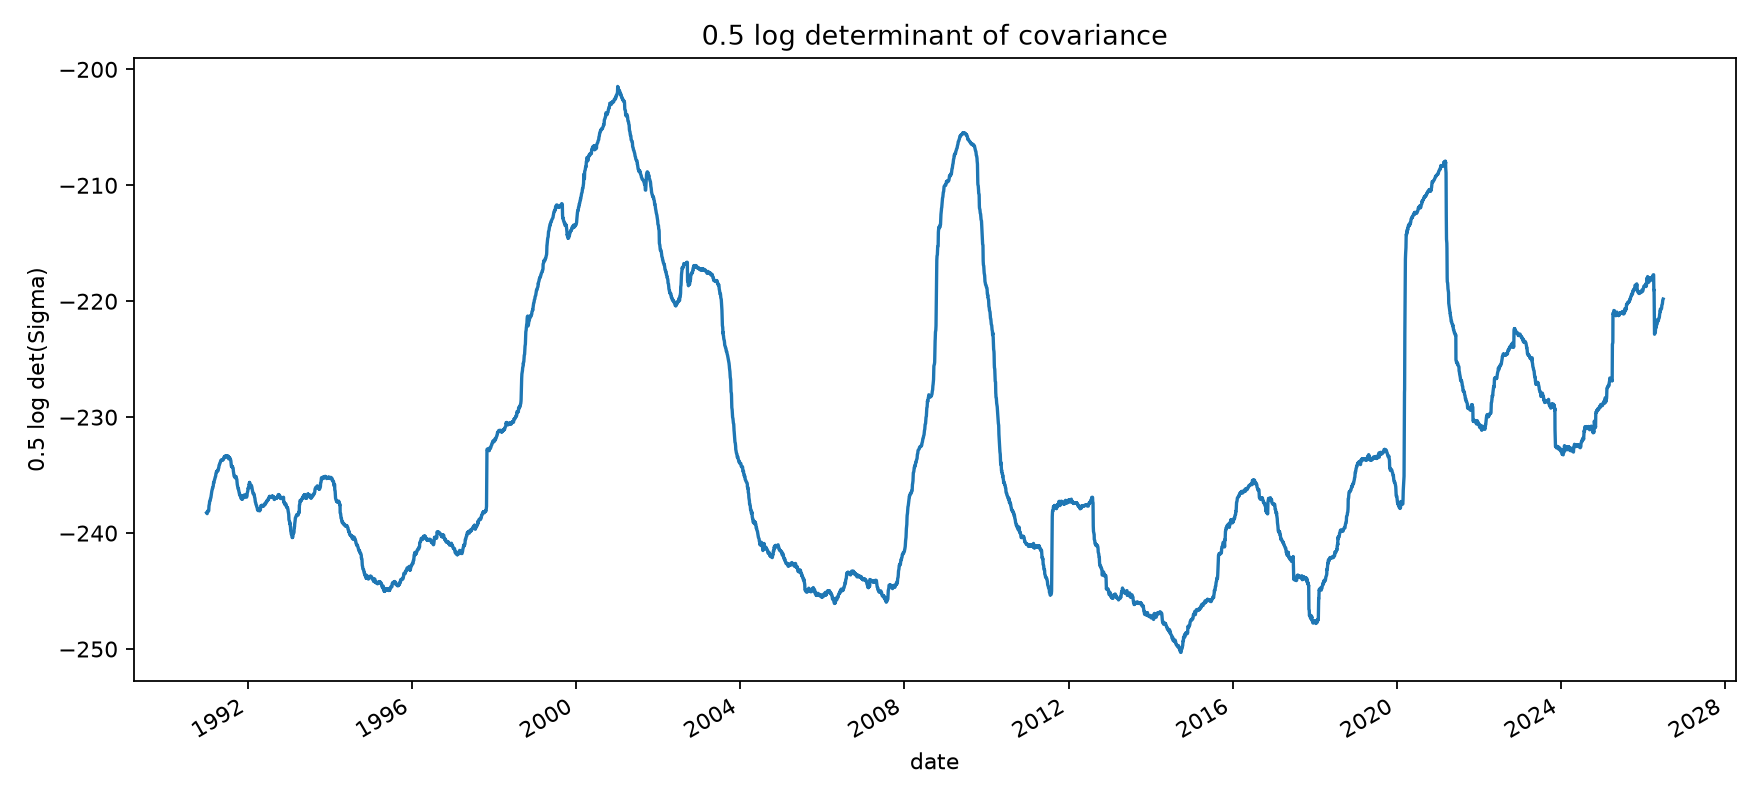
\includegraphics[width=\linewidth]{figures/ff49_logdet_covariance.png}
\caption{FF49: $H^{cov}_t=\tfrac12\log\det\Sigma_t$. Visible drops coincide with the stress episodes listed above (2000--2002, 2008, 2020, 2022).}
\label{fig:ff49-logdet}
\end{figure}

Figure~\ref{fig:ff49-logdet} plots the level series whose stability is at stake: $H^{cov}_t$ ranges from a maximum of $-201.5$ (January 2001, a low-volatility, low-dependence regime) to a minimum of $-250.3$ (September 2014, a calm period with unusually tight cross-industry dependence — a reminder that a low $\det\Sigma_t$ is not synonymous with a crisis; it can also reflect a quiet market where industries move together for structural reasons). The largest \emph{single-day} drops in $\Delta H^{cov}$, however, do not line up cleanly with the crisis list; several of the sharpest one-day contractions (e.g.\ 2021-03, 2021-06, 2023-11) occur outside any labelled stress episode. This is a known artefact of fixed-length rolling windows: a jump can be produced by an extreme observation entering \emph{or} leaving the 252-day window rather than by anything happening in the market on that specific day. The regime-level statistics reported for H1--H2 (which average over hundreds of stress dates) are robust to this edge effect; a reading of individual daily spikes in $\Delta H^{cov}$ as dated "events" is not, and the paper does not rely on such a reading.

\paragraph{Does compensation hold within, and not just across, crises?} Averaging over all 894 stress dates gives $\operatorname{corr}(\Delta H^{vol},\Delta H^{dep})=-0.40$, but this pools episodes that are, on inspection, quite different. Restricting to the 2008 window (August--December 2008) gives $\operatorname{corr}=-0.61$, close to the calm-regime value — compensation held up well through the global financial crisis. Restricting to the acute COVID crash (mid-February to mid-April 2020) gives $\operatorname{corr}=-0.02$: during those eight weeks $H^{vol}$ and $H^{dep}$ moved with no measurable offsetting relationship at all, and $H^{cov}$ barely net-changed over the window ($-237.46\to-237.51$) only because a sharp initial contraction was later reversed, not because the two components offset each other day by day. A plausible reading is that 2008 was a slow-building, rotating stress (credit and liquidity conditions deteriorating unevenly across industries, leaving room for cross-sectional reallocation) whereas COVID was a simultaneous, economy-wide shock that pushed volatility up and correlations up together with little room for the dependence structure to do anything but track volatility. This heterogeneity is itself a substantive, and previously unstated, qualification of H2: the compensation regularity is real on average but is not a universal law of stress episodes, and future work should treat "type of shock" (idiosyncratic/rotating vs.\ systemic/simultaneous) as a moderator rather than folding all stress dates into one bucket.

\paragraph{What this contributes to the paper's argument.} The theoretical results (Sections 2--6) establish what maximum entropy proves; nothing in this section is needed to establish those. What Figures~\ref{fig:ff49-components}--\ref{fig:ff49-logdet} and the statistics around them add is evidence that the \emph{empirical} hypothesis motivating the covariance-entropy decomposition — that marginal-volatility and dependence entropy partially offset during stress — is not merely plausible but measurable and repeatable on 36 years of the intended dataset: a $56.7\%$ variance reduction, a significant negative slope with $R^2\approx0.4$, and directional agreement with an unrelated dataset (Section~\ref{sec:pilot}) are the kind of evidence a purely theoretical argument cannot supply. Equally, the COVID-vs-2008 asymmetry and the null out-of-sample result for H3 are evidence \emph{against} overstating the hypothesis: the paper's proof burden for H2 is "a real, partial, regime-dependent tendency," and that is what the data show — not more.

\section{Robustness check on a second, independent real dataset}
\label{sec:pilot}
As a second, independent check — collected before the FF49 file was obtained, and left in place as a robustness diagnostic on an unrelated market and period — the identical pipeline (rolling Ledoit--Wolf covariance, entropy decomposition, stress regime, predictive regression) was run unmodified on the \texttt{EuStockMarkets} panel (Bollerslev and Ghysels), the daily closing levels of the DAX, SMI, CAC and FTSE indices, 1{,}860 contemporaneous trading days from 1991-01-02 through 1998-12-31, obtained from the public Rdatasets mirror (\texttt{config/pilot\_eu\_stock\_markets.yaml}). This is a $N=4$, single-window pilot, not a substitute for the $N=48$ result above.

With a 252-day rolling window and the top decile of trailing 21-day market volatility as the stress indicator (161 of 1{,}608 rolling dates, clustering around the September 1992 ERM crisis, the September 1993 ERM turbulence and the October--November 1997 Asian-crisis episode):
\begin{itemize}
\item \textbf{H1.} Stress dates show higher marginal volatility ($H^{vol}=-18.25$ vs.\ $-18.93$ in calm dates) and lower $\det R$, i.e.\ lower $H^{dep}$ ($-1.147$ vs.\ $-0.911$). Both effects point in the direction H1 predicts.
\item \textbf{H2.} $\operatorname{corr}(\Delta H^{vol},\Delta H^{dep})=-0.23$ over the full sample: negative, as the compensation hypothesis requires. In the stress subsample, $\operatorname{sd}(\Delta H^{cov})=0.0210$ is below the value implied by treating the two components as uncorrelated, $\sqrt{\operatorname{sd}(\Delta H^{vol})^2+\operatorname{sd}(\Delta H^{dep})^2}=0.0315$, consistent with partial (not exact) compensation. In variance terms, $\operatorname{Var}(\Delta H^{cov})$ is $17.6\%$ below the uncorrelated-components benchmark over the full sample — the same effect as in FF49, but roughly a third the size ($17.6\%$ vs.\ $56.7\%$).
\item \textbf{H3.} Adding $H^{dep}$ to $H^{vol}$ lowers 21-day-ahead realized-volatility test MSE only marginally (0.0849 vs.\ 0.0869) and the coefficient on $H^{dep}$ is not significant on the 70/30 split ($p=0.64$). With $N=4$ assets and one non-overlapping regime cycle, this pilot is underpowered for H3; it neither confirms nor refutes the predictive-value hypothesis.
\end{itemize}
Both datasets agree on the sign and qualitative shape of H1 and H2, on two disjoint asset universes, time spans and market structures; this cross-dataset agreement is itself modest additional evidence that the compensation effect is not an artifact of the FF49 construction. Neither dataset supports H3 out of sample under the simple linear specification used here.

\begin{figure}[htbp]
\centering
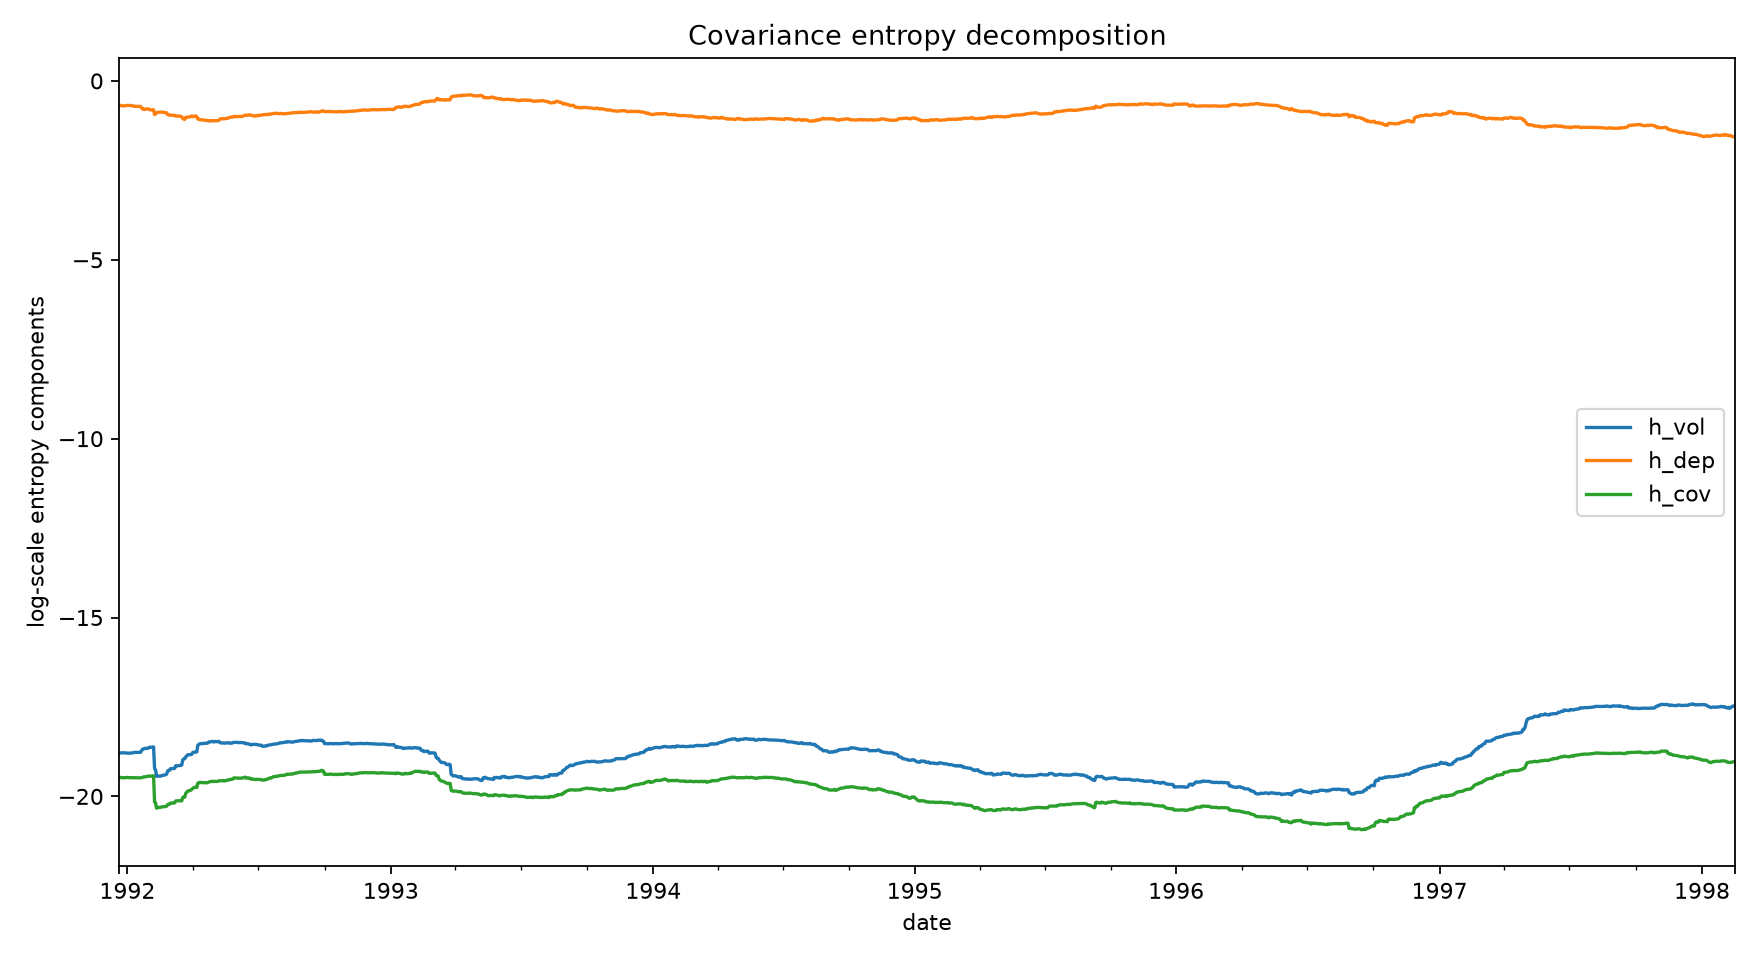
\includegraphics[width=\linewidth]{figures/pilot_entropy_components.png}
\caption{EuStockMarkets, 1991--1998: rolling $H^{vol}$, $H^{dep}$ and $H^{cov}$ (252-day window, $N=4$). Same qualitative pattern as Figure~\ref{fig:ff49-components} on an unrelated market and period.}
\label{fig:pilot-components}
\end{figure}

Figure~\ref{fig:pilot-components} shows the same anti-phased pattern as Figure~\ref{fig:ff49-components} — $H^{vol}$ and $H^{dep}$ move in opposite directions around the 1992 ERM and 1997 Asian-crisis episodes, and $H^{cov}$ sits in a visibly tighter band than either component — but the effect is plainly less pronounced: the three lines are closer together throughout, consistent with the smaller ($17.6\%$ vs.\ $56.7\%$) variance reduction. With only $N=4$ indices there are only $4\times3/2=6$ pairwise correlations available to reallocate risk into, against $48\times47/2=1{,}128$ for FF49; if the compensation mechanism works by redistributing risk across a cross-section, a larger cross-section mechanically gives it more room to operate, which is a natural candidate explanation for the size gap and a testable prediction in itself (compensation strength should scale with $N$) that neither dataset alone can confirm.

\begin{figure}[htbp]
\centering
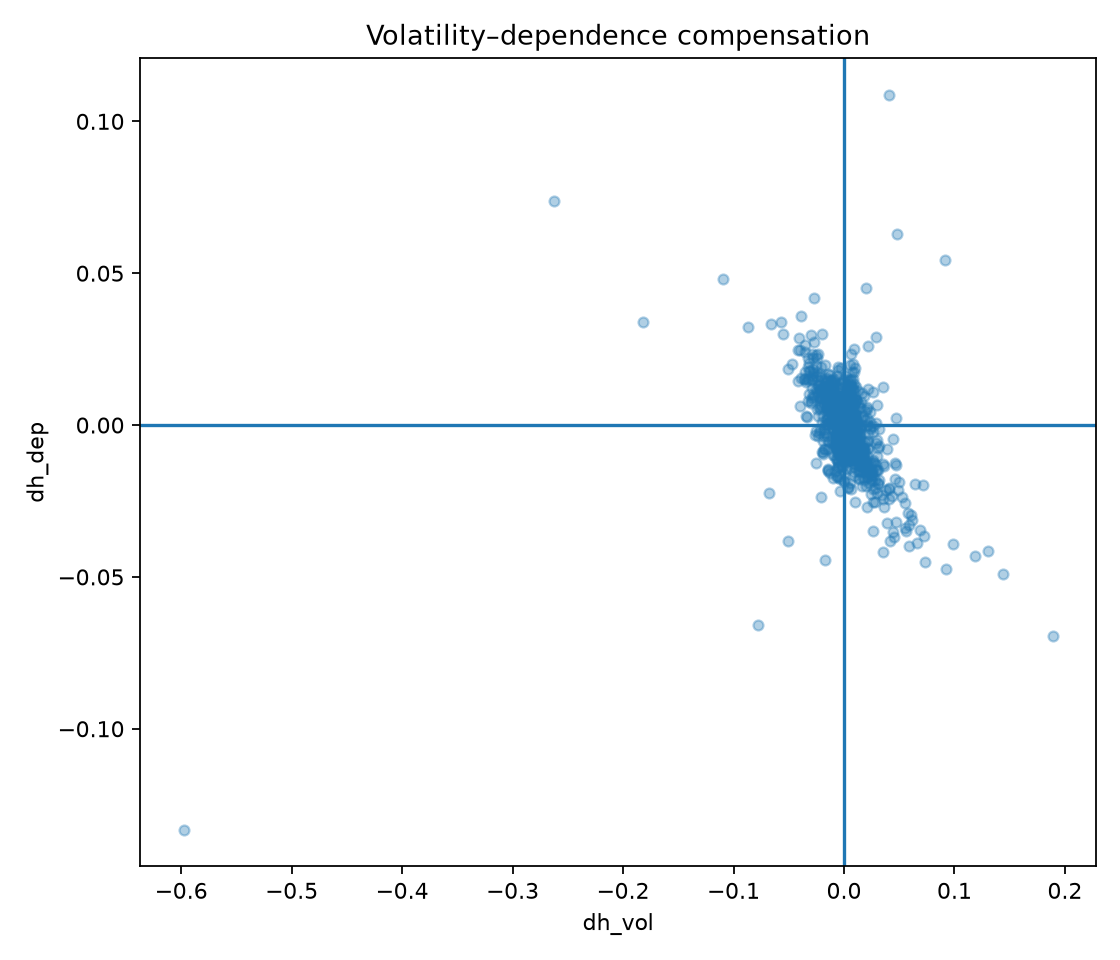
\includegraphics[width=0.8\linewidth]{figures/pilot_compensation_scatter.png}
\caption{EuStockMarkets: $\Delta H^{dep}_t$ against $\Delta H^{vol}_t$, corresponding to $\operatorname{corr}(\Delta H^{vol},\Delta H^{dep})=-0.23$.}
\label{fig:pilot-scatter}
\end{figure}

The corresponding OLS fit is $\Delta H^{dep}_t\approx-0.108\,\Delta H^{vol}_t$ with $R^2=0.052$ — a much shallower slope and a much noisier cloud than Figure~\ref{fig:ff49-scatter} ($R^2=0.398$), visually confirming that the linear relationship, while same-signed, explains an order of magnitude less of the day-to-day variation here than in FF49. Taken together with the variance-reduction gap, the two figures support a consistent story across both datasets: the sign of the compensation effect replicates out of sample (different market, different decade, different number of assets), but its \emph{strength} does not — it is markedly weaker on a 4-asset panel than on a 48-asset one. That combination (sign replicates, magnitude does not) is exactly what the paper can honestly claim as evidence: it argues for compensation being a genuine, cross-sectionally scalable phenomenon rather than a statistical fluke of one dataset, without overstating what a 4-asset, single-window pilot can establish on its own.

\section{Non-Gaussianity and relative entropy}
The Gaussian reference distribution is not assumed to equal the empirical distribution. Applying the identity from the proof of Proposition~1 date-by-date: if $q_t$ is the Gaussian distribution matching the empirical mean and covariance at $t$ and $p_t$ is the true empirical density, then
\[
D_{KL}(p_t\Vert q_t)=h(q_t)-h(p_t)\ge0.
\]
This suggests a useful robustness extension: separate covariance-volume dynamics ($h(q_t)$, driven entirely by $\Sigma_t$) from time variation in $D_{KL}(p_t\Vert q_t)$, i.e.\ from how far the conditional return distribution is from Gaussian at each date. A stress episode could in principle show compensation in $h(q_t)$ while simultaneously showing rising $D_{KL}(p_t\Vert q_t)$ (fatter tails, more skewness) that the covariance-only decomposition does not capture.

\section{Risk-neutral interpretation}
The maximum-entropy argument is naturally a physical-measure statement. Under $\mathbb P$,
\[
\frac{dS_t}{S_t}=\mu_t^{\mathbb P}dt+\sigma_tdW_t^{\mathbb P}.
\]
Under $\mathbb Q$ for a non-dividend-paying asset,
\[
\frac{dS_t}{S_t}=r_tdt+\sigma_tdW_t^{\mathbb Q}.
\]
Maximum entropy under historical constraints does not by itself determine a risk-neutral pricing measure or option prices.

\section{Limitations}
The principal limitations are non-Gaussian tails, stochastic volatility, unstable dependence, finite-sample covariance error, and the unit dependence of differential entropy. In addition, industry portfolios are not independent firms and can mechanically display common-factor dependence. A future individual-stock analysis using CRSP/WRDS would therefore be a valuable robustness test. The pilot illustration in Section~\ref{sec:pilot} carries its own, additional limitations: $N=4$ is too small to give the covariance-determinant a meaningful ``volume'' interpretation, the sample spans a single 8-year window with essentially one stress cycle, and dates are reconstructed from a business-day count rather than the true exchange calendar.

The FF49 result in Section~\ref{sec:ff49results} has its own specific caveat for H3: the 252-day rolling window means consecutive $H^{vol}_t,H^{dep}_t$ observations share 251 of 252 underlying return days, and the 21-day forecast target is itself an overlapping sum. This heavy overlap inflates the effective persistence of every series involved and is only partially addressed by the HAC standard errors used here (21 lags); it most plausibly explains why $H^{dep}$ is highly significant in sample but does not reduce out-of-sample MSE. A more decisive H3 test would re-estimate at a non-overlapping frequency (e.g.\ one observation per 21-day block), use an expanding or rolling walk-forward evaluation rather than a single 70/30 split, and compare against a GARCH/DCC benchmark rather than only the volatility-only OLS baseline used here.

\section{References}
\begin{itemize}
\item Jaynes, E. T. (1957). Information Theory and Statistical Mechanics. \textit{Physical Review}, 106, 620--630.
\item Black, F. and Scholes, M. (1973). The Pricing of Options and Corporate Liabilities. \textit{Journal of Political Economy}, 81(3), 637--654.
\item Merton, R. C. (1973). Theory of Rational Option Pricing. \textit{Bell Journal of Economics and Management Science}, 4(1), 141--183.
\item Engle, R. (2002). Dynamic Conditional Correlation: A Simple Class of Multivariate Generalized Autoregressive Conditional Heteroskedasticity Models. \textit{Journal of Business \& Economic Statistics}, 20(3), 339--350.
\item Ledoit, O. and Wolf, M. (2004). A Well-Conditioned Estimator for Large-Dimensional Covariance Matrices. \textit{Journal of Multivariate Analysis}, 88(2), 365--411.
\item Fama, E. F. and French, K. R. Kenneth French Data Library, 49 Industry Portfolios.
\item Bollerslev, T. and Ghysels, E. (1996). Periodic Autoregressive Conditional Heteroscedasticity. \textit{Journal of Business \& Economic Statistics}, 14(2), 139--151. (Source of the EuStockMarkets pilot series, mirrored at https://github.com/vincentarelbundock/Rdatasets.)
\end{itemize}

\section{Conclusion}
The theoretical contribution is a clean separation between what maximum entropy proves and what financial modelling assumes. Fixed first and second moments imply a Gaussian maximum-entropy distribution. Temporal assumptions then produce Brownian diffusion, and exponentiation produces GBM. The empirical proposal is different: the covariance determinant may display partial compensation between marginal volatility and dependence-induced contraction. On the FF49 industry cross-section (Section~\ref{sec:ff49results}), that compensation is real and economically sizeable: stress raises marginal volatility and contracts $\det R$ (H1), and the two entropy components move in strongly offsetting directions, leaving covariance-volume markedly more stable than either alone (H2). A second, unrelated real dataset (Section~\ref{sec:pilot}) replicates the sign of both effects. Turning this stability into a standalone volatility forecast (H3) is not yet supported out of sample and is left as an open question, most likely requiring a genuine walk-forward evaluation and a non-overlapping estimation frequency rather than the simple 70/30 chronological split used here.

\end{document}
